\documentclass{beamer}

\usepackage[T1]{fontenc}
\usepackage[utf8]{inputenc}
\usepackage[polish]{babel}
\usepackage{lmodern}

\usepackage{tikz}
\usetikzlibrary{positioning, arrows.meta, fit}


\usetheme{Madrid}
\usecolortheme{default}

%------------------------------------------------------------
%This block of code defines the information to appear in the
%Title page
\title[Odczyt tablicy rejestracyjnej]{Odczytywanie tablicy rejestracyjnej ze zdjęcia}

\subtitle{Deep learning w Chmurze}

\author{Joanna Dagil \and Maja Szerszeń}

\date{\today}

%\logo{\includegraphics[height=1cm]{overleaf-logo}}

%End of title page configuration block
%------------------------------------------------------------



%------------------------------------------------------------
%The next block of commands puts the table of contents at the 
%beginning of each section and highlights the current section:

%\AtBeginSection[]
%{
%  \begin{frame}
%    \frametitle{Spis treści}
%    \tableofcontents[currentsection]
%  \end{frame}
%}
%------------------------------------------------------------


\begin{document}

%The next statement creates the title page.
\frame{\titlepage}


%---------------------------------------------------------
%This block of code is for the table of contents after
%the title page
\begin{frame}
\frametitle{Spis treści}
\tableofcontents
\end{frame}
%---------------------------------------------------------


\section{Streszczenie}

\begin{frame}{Streszczenie}
Dwustopniowy model: YOLO + własna sieć CNN.

albo gotowy model OCR
\end{frame}



%---------------------------------------------------------


%---------------------------------------------------------

\section{Wstęp / wprowadzenie}

\begin{frame}{Wstęp / wprowadzenie}

Model składa się z dwóch głównych części:

\begin{itemize}
    \item wykrywania położenia tablicy rejestracyjnej przy użyciu modelu YOLO11n,
    \item odczytywania tekstu z wyciętego obszaru tablicy przy użyciu modułu OCR.
\end{itemize}

\end{frame}

%---------------------------------------------------------


%---------------------------------------------------------
\section{Opis kontekstu i celu projektu}


\begin{frame}{Opis kontekstu i celu projektu}

\end{frame}

%---------------------------------------------------------


%---------------------------------------------------------
\section{Literatura}

\begin{frame}{Literatura}

\small

\begin{itemize}
    \item Khanam, R., Hussain, M. (2024). 
    \textit{YOLOv11: An Overview of the Key Architectural Enhancements}. 
    arXiv:2410.17725.\\
    \url{https://arxiv.org/abs/2410.17725}

    \item Jocher, G., Qiu, J. (2024). 
    \textit{Ultralytics YOLO11} (Version 11.0.0) [Computer software]. 
    GitHub.\\
    \url{https://github.com/ultralytics/ultralytics}
\end{itemize}

\end{frame}
%---------------------------------------------------------


%---------------------------------------------------------
\section{Opis danych}





%---------------------------------------------------------


%---------------------------------------------------------

\begin{frame}{Opis danych}

\begin{columns}

\column{0.60\textwidth}

\textit{License Plate Detection Dataset (10,125 Images)}, zawierający zdjęcia pojazdów z oznaczonym położeniem tablic rejestracyjnych.

\vspace{0.2cm}

Dane są zapisane w formacie zgodnym z YOLO.  
Dla każdego obrazu istnieje odpowiadający mu plik tekstowy z etykietą.

\column{0.40\textwidth}

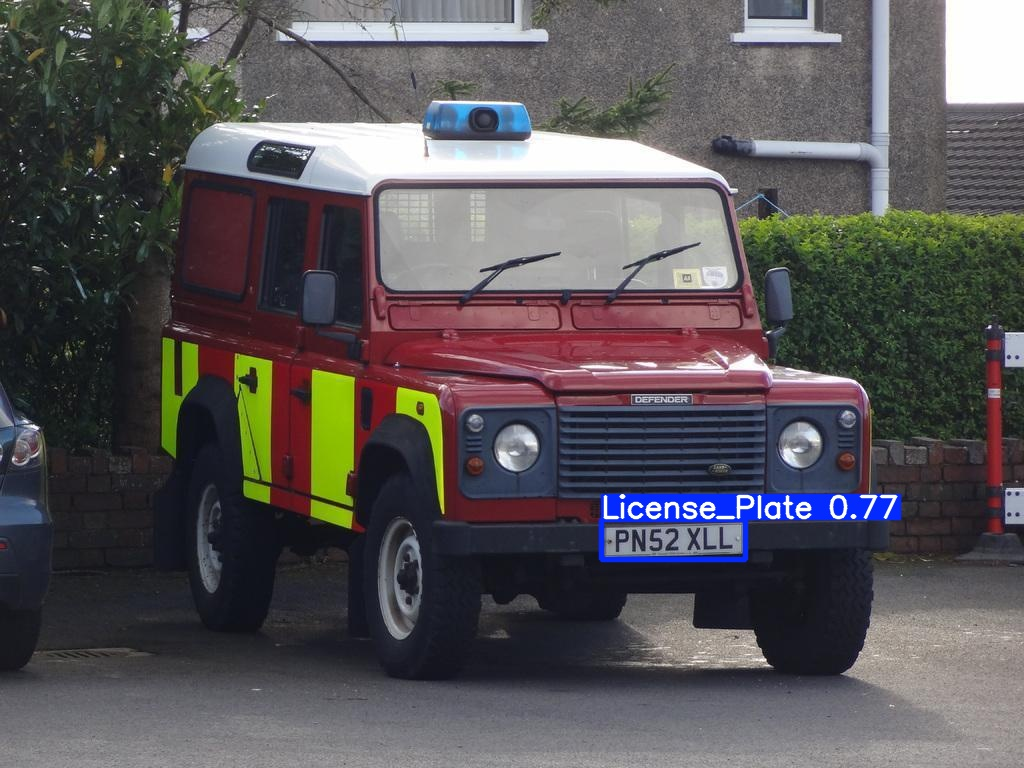
\includegraphics[width=\textwidth]{pics/TODO-car-wo-label.jpeg}

\vspace{0.2cm}

\end{columns}



\begin{center}
\begin{tikzpicture}[
    every node/.style={font=\scriptsize},
    num/.style={font=\ttfamily\large},
    def/.style={align=center, font=\scriptsize},
    arrow/.style={-Latex, thin}
]

% Numbers in the example label
\node[num] (class) at (0,0) {0};
\node[num] (xc)    at (1.2,0) {0.512};
\node[num] (yc)    at (2.8,0) {0.781};
\node[num] (w)     at (4.4,0) {0.154};
\node[num] (h)     at (6.0,0) {0.067};

% Definitions alternating above and below
\node[def, above=0.5cm of class] (classdef) {klasa obiektu};
\node[def, below=0.5cm of xc]    (xcdef)    {\texttt{x\_center}\\środek w poziomie};
\node[def, above=0.5cm of yc]    (ycdef)    {\texttt{y\_center}\\środek w pionie};
\node[def, below=0.5cm of w]     (wdef)     {\texttt{width}\\szerokość ramki};
\node[def, above=0.5cm of h]     (hdef)     {\texttt{height}\\wysokość ramki};

% Vertical arrows
\draw[arrow] (classdef) -- (class);
\draw[arrow] (xc) -- (xcdef);
\draw[arrow] (ycdef) -- (yc);
\draw[arrow] (w) -- (wdef);
\draw[arrow] (hdef) -- (h);

\end{tikzpicture}
\end{center}


\scriptsize
Wartości \texttt{x\_center}, \texttt{y\_center}, \texttt{width} i \texttt{height}
są znormalizowane do rozmiaru obrazu, czyli mają wartości od 0 do 1.

\end{frame}

%---------------------------------------------------------

\begin{frame}{Opis danych}

    The dataset contains bounding-box annotations for license plate locations, which allows quantitative evaluation of the detection model. However, it does not contain ground-truth license plate transcriptions, so OCR results were assessed qualitatively on selected examples.

Dataset \textit{License Plate Detection Dataset (10,125 Images)}  zawiera adnotacje lokalizacji tablic na zdjęciu, które pozwalają na detekcję tablicy na obrazie. Nie zawierają jednakże oznaczenia faktycznych numerów tablic. W celu zmierzenia accuracy odczytywania numerów posłużymy się analizą jakościową na małej próbce ręcznie oznaczonych tablic.

\end{frame}


%---------------------------------------------------------

%---------------------------------------------------------


\section{Opis metod}

\begin{frame}{Opis metod}

\begin{columns}[T,onlytextwidth]

% LEWA KOLUMNA
\column{0.52\textwidth}

\small
W projekcie zastosowano podejście dwustopniowe, ponieważ problem odczytywania tablicy rejestracyjnej składa się z dwóch zadań:

\begin{itemize}
    \item \textbf{detekcji tablicy} -- znalezienia miejsca, w którym tablica znajduje się na obrazie,
    \item \textbf{rozpoznania tekstu} -- odczytania znaków z wyciętego fragmentu tablicy.
\end{itemize}

% PRAWA KOLUMNA
\column{0.46\textwidth}

\centering

\resizebox{0.9\textwidth}{!}{
\begin{tikzpicture}[
    node distance=0.35cm,
    box/.style={
        rectangle,
        rounded corners,
        draw=blue!60,
        fill=blue!8,
        thick,
        minimum width=3.8cm,
        minimum height=0.65cm,
        align=center,
        font=\scriptsize
    },
    arrow/.style={
        -Latex,
        thick,
        draw=blue!70
    },
    stagebox/.style={
        rectangle,
        rounded corners,
        draw=gray!70,
        dashed,
        thick,
        inner sep=0.18cm
    },
    stagelabel/.style={
        font=\scriptsize\bfseries,
        rotate=90,
        text=gray!80
    }
]

\node[box] (image) {Obraz pojazdu};
\node[box, below=of image] (plateyolo) {YOLO -- detekcja tablicy};
\node[box, below=of plateyolo] (crop) {Crop tablicy};
\node[box, below=of crop] (charyolo) {YOLO -- klasyfikacja znaków};
\node[box, below=of charyolo] (filter) {Filtrowanie detekcji};
\node[box, below=of filter] (sort) {Sortowanie znaków};
\node[box, below=of sort] (text) {Odczytany tekst};

\draw[arrow] (image) -- (plateyolo);
\draw[arrow] (plateyolo) -- (crop);
\draw[arrow] (crop) -- (charyolo);
\draw[arrow] (charyolo) -- (filter);
\draw[arrow] (filter) -- (sort);
\draw[arrow] (sort) -- (text);

% Przerywane ramki etapów
\node[stagebox, fit=(image)(plateyolo)(crop)] (stage1) {};
\node[stagebox, fit=(charyolo)(filter)(sort)(text)] (stage2) {};

% Pionowe etykiety etapów
\node[stagelabel, right=0.15cm of stage1] {Etap 1};
\node[stagelabel, right=0.15cm of stage2] {Etap 2};

\end{tikzpicture}
}

\end{columns}

\end{frame}



%---------------------------------------------------------
\begin{frame}{YOLO11n}

Do wykrywania położenia tablicy rejestracyjnej wykorzystano model \texttt{YOLO11n} z biblioteki Ultralytics.

\begin{itemize}
    \item YOLO jest jednofazowym modelem detekcji obiektów.
    \item W projekcie model uczony był detekcji jednej klasy: \texttt{License\_Plate}.
    \item Model analizuje cały obraz i zwraca ramki ograniczające, czyli \textit{bounding box}, oraz poziom pewności detekcji, czyli \textit{confidence score} dla wykrytych obiektów.
    \item Zastosowano wariant \texttt{YOLO11n}, ponieważ jest lekki i szybki, co ułatwia eksperymenty w środowisku chmurowym.
\end{itemize}

\end{frame}
%---------------------------------------------------------
\begin{frame}{Crop tablicy i OCR}

Po wykryciu tablicy przez model YOLO wycinany jest fragment obrazu odpowiadający przewidzianej ramce ograniczającej.

\begin{itemize}
    \item Crop pozwala ograniczyć OCR tylko do obszaru tablicy.
    \item Dzięki temu moduł OCR nie analizuje całego zdjęcia, lecz jedynie fragment zawierający znaki rejestracji.
    \item Do odczytu tekstu wykorzystano OCR, który zwraca przewidywany ciąg znaków oraz confidence score.
    \item Wynik OCR został poddany prostemu postprocessingowi: usunięto spacje, znaki specjalne oraz zamieniono litery na wielkie.
\end{itemize}

\end{frame}
%---------------------------------------------------------
\begin{frame}{Postprocessing wyniku}

Wyniki OCR mogą zawierać dodatkowe znaki, spacje lub błędy wynikające z jakości obrazu. Dlatego zastosowano prosty etap czyszczenia tekstu.

\begin{itemize}
    \item Zamiana wszystkich liter na wielkie.
    \item Usunięcie spacji i znaków specjalnych.
    \item Pozostawienie wyłącznie liter i cyfr.
    \item Porównanie wyników OCR na przykładach wizualnych.
\end{itemize}

\begin{center}
\texttt{"PCZ DSq8"} $\rightarrow$ \texttt{"PCZDSQ8"}
\end{center}

\end{frame}
%---------------------------------------------------------

%---------------------------------------------------------

\section{Opis wdrożenia metod / modelu}

\begin{frame}{Opis wdrożenia metod / modelu}
    
\end{frame}

%---------------------------------------------------------


\section{Opis wdrożenia metod / modelu}

\begin{frame}{Opis wdrożenia metod / modelu}

Wdrożenie modelu zostało zrealizowane w środowisku notebookowym z wykorzystaniem biblioteki Ultralytics YOLO oraz modułu OCR.

\begin{itemize}
    \item Dane zostały pobrane z Kaggle przy użyciu biblioteki \texttt{kagglehub}.
    \item Zbiór danych zapisano w formacie zgodnym z YOLO, wykorzystując plik konfiguracyjny \texttt{data.yaml}.
    \item Do detekcji tablic rejestracyjnych użyto modelu \texttt{YOLO11n}.
    \item Model został wytrenowany na obrazach pojazdów z oznaczonymi ramkami tablic.
    %\item Po treningu zapisano najlepszy model w pliku \texttt{best.pt}.
    \item Następnie model wykorzystano do predykcji na obrazach testowych.
\end{itemize}

\end{frame}

%---------------------------------------------------------


\begin{frame}{Pipeline działania modelu}

Cały proces działania modelu składa się z kilku etapów:

\begin{center}
\texttt{obraz} $\rightarrow$ \texttt{detekcja YOLO} $\rightarrow$ \texttt{crop tablicy} $\rightarrow$ \texttt{OCR} $\rightarrow$ \texttt{tekst}
\end{center}

\begin{itemize}
    \item Najpierw model YOLO wykrywa położenie tablicy rejestracyjnej na obrazie.
    \item Na podstawie wykrytej ramki ograniczającej wycinany jest fragment obrazu zawierający tablicę.
    \item Wycięty fragment jest przekazywany do modułu OCR.
    \item Wynik OCR jest czyszczony przez usunięcie spacji, znaków specjalnych oraz zmianę liter na wielkie.
    \item Końcowym wynikiem jest przewidywany tekst tablicy rejestracyjnej.
\end{itemize}

\end{frame}

%---------------------------------------------------------


\begin{frame}{Trening i zapis modelu}

Model trenowano z wykorzystaniem transfer learning'u na bazie gotowych wag \texttt{yolo11n.pt}.

\begin{itemize}
    \item Obrazy wejściowe były przeskalowywane do ustalonego rozmiaru, np. \texttt{640 $\times$ 640}.
    \item Podczas treningu monitorowano funkcję straty oraz metryki detekcji.
    \item Po zakończeniu treningu YOLO automatycznie zapisał dwa warianty modelu:
    \begin{itemize}
        \item \texttt{best.pt} -- model z najlepszym wynikiem na zbiorze walidacyjnym,
        \item \texttt{last.pt} -- model z ostatniej epoki treningu.
    \end{itemize}
    \item Do dalszej ewaluacji i predykcji wykorzystano model \texttt{best.pt}.
\end{itemize}

\end{frame}

%---------------------------------------------------------


\begin{frame}{Ewaluacja i predykcja}

Po treningu model został oceniony na zbiorze walidacyjnym oraz testowym.

\begin{itemize}
    \item Dla części detekcyjnej wykorzystano metryki:
    \begin{itemize}
        \item \textit{precision} -- precyzja wykrytych ramek,
        \item \textit{recall} -- odsetek poprawnie znalezionych tablic,
        \item \textit{mAP@0.5} -- jakość detekcji przy progu IoU równym 0.5,
        \item \textit{mAP@0.5:0.95} -- bardziej rygorystyczna wersja mAP.
    \end{itemize}
    \item Dodatkowo zapisano przykładowe obrazy z przewidywanymi ramkami.
    \item Dla wybranych obrazów wykonano crop tablicy oraz odczyt tekstu za pomocą OCR.
\end{itemize}

\end{frame}


%---------------------------------------------------------


%---------------------------------------------------------

\section{Wyniki}


\begin{frame}{Wyniki}

    
\end{frame}


%---------------------------------------------------------


%---------------------------------------------------------
\section{Wnioski}


\begin{frame}{Wnioski}

    
\end{frame}




%---------------------------------------------------------
%Changing visivility of the text
\begin{frame}
\frametitle{Sample frame title}
This is a text in second frame. For the sake of showing an example.

\begin{itemize}
    \item<1-> Text visible on slide 1
    \item<2-> Text visible on slide 2
    \item<3> Text visible on slides 3
    \item<4-> Text visible on slide 4
\end{itemize}
\end{frame}

%---------------------------------------------------------


%---------------------------------------------------------
%Example of the \pause command
\begin{frame}
In this slide \pause

the text will be partially visible \pause

And finally everything will be there
\end{frame}
%---------------------------------------------------------


%---------------------------------------------------------
%Highlighting text
\begin{frame}
\frametitle{Sample frame title}

In this slide, some important text will be
\alert{highlighted} because it's important.
Please, don't abuse it.

\begin{block}{Remark}
Sample text
\end{block}

\begin{alertblock}{Important theorem}
Sample text in red box
\end{alertblock}

\begin{examples}
Sample text in green box. The title of the block is ``Examples".
\end{examples}
\end{frame}
%---------------------------------------------------------


%---------------------------------------------------------
%Two columns
\begin{frame}
\frametitle{Two-column slide}

\begin{columns}

\column{0.5\textwidth}
This is a text in first column.
$$E=mc^2$$
\begin{itemize}
\item First item
\item Second item
\end{itemize}

\column{0.5\textwidth}
This text will be in the second column
and on a second tought this is a nice looking
layout in some cases.
\end{columns}
\end{frame}
%---------------------------------------------------------


\end{document}